\chapter{Обзор предметной области} \label{ch1}

В данной главе рассмотрены основные методы обеспечения безопасности объектов в условиях современных угроз. Описаны различные формы охраны, такие как государственная, ведомственная и вневедомственная, а также способы организации охраны объектов по периметру и внутри территории. Особое внимание уделено существующим инженерно-техническим средствам охраны, системам видеонаблюдения, контроля доступа и сигнализации. Также подробно проанализированы технические средства обнаружения несанкционированного доступа. В заключение представлены выводы о необходимости разработки автономных интеллектуальных методов охраны территорий для повышения уровня безопасности\cite{obespech-bezopasnosti}.


\section{Задача обеспечения безопасности} \label{ch1:sec1}

В современных условиях резкого осложнения криминогенной обстановки, роста числа террористических и диверсионных актов проблема обеспечения безопасности объектов входит в разряд приоритетных задач, как для государственных организаций, так и для организаций любой другой формы собственности и для собственников любых видов недвижимости.

По субъектам организации охранной деятельности различаются:
\begin{itemize}
    \item государственная охрана, представляющая собой специализированные автономные организационные структуры, предназначенные для охраны объектов особой государственной важности, перечень которых устанавливается специальными нормативными актам правительства;
    \item ведомственная охрана, представляет собой специализированные, вооруженные (как правило) подразделения, осуществляющие охрану различных объектов, входящих в структуру определенного ведомства;
    \item вневедомственная охрана это специализированные подразделения, осуществляющие охрану объектов, принадлежащих различным ведомствам и частным лицам, на контрактной, возмездной основе.
\end{itemize}

Формы организации, номенклатура охранных услуг, методы и средства реализации охранной деятельности в основном определяются тем, какому субъекту охранной деятельности подведомственен данный объект, кем он охраняется - государством, ведомством, вневедомственной государственной или частной охраной.

На подступах к объектам охраны создаются активные и пассивные защитные препятствия, например: система физических препятствий (инженерные заграждения), специальное оборудование мест хранения секретных документов, контрразведывательное обеспечение.

Надежность охраны достигается детальным построением системы охраны, правильной организацией и бдительным несением службы нарядами.

В зависимости от местности, характера и категории объекта и других особенностей охрана объектов может быть организована следующими способами:
\begin{enumerate}[1.]
    \item По периметру. Технические средства охраны выставляются на границе охраняемой территории и преграждают доступ к объекту вне пропускных пунктов (именно таким способом, как правило, охраняются некоторые режимные объекты).
    \item По отдельным объектам. Личный состав выставляется непосредственно на охраняемом объекте (примером такого способа охраны может быть порядок организации охраны складов МВД по хранению боеприпасов).
    \item Смешанным способом. По периметру и отдельным объектам одновременно.
    \item Способом оперативного дежурства. Охранные функции осуществляются комплексом инженерно-технических средств охраны при дежурном состоянии сил охраны (примером такого способа охраны является организация охраны любой атомной электростанции).
\end{enumerate}

На основе изученных статистических данных, можно сделать вывод, что охраняемые объекты наиболее часто подвергаются следующим видам угроз:
\begin{itemize}
    \item несанкционированное проникновение на территорию;
    \item несанкционированное получение информации об объекте или иной закрытой информации путем установки на объекте скрытых средств негласного получения информации;
    \item нападение на охраняемый объект с целью хищения материальных ценностей;
    \item угрозы жизни и здоровью персонала и посетителей объекта, в том числе взятие заложников с целью достижения иных целей;
    \item нарушение инфраструктуры и линий жизнеобеспечения объекта охраны;
    \item нарушение режима работы объекта, с целью прекращения его функционирования;
    \item саботаж технических средств охраны.
\end{itemize}


\section{Существующие методы обеспечения безопасности} \label{ch1:sec2} 

Методы обеспечения безопасности объектов включают в себя широкий спектр мер, направленных на предотвращение и минимизацию рисков, связанных с несанкционированным доступом, диверсиями, террористическими актами и другими угрозами. Рассмотрим основные существующие методы обеспечения безопасности.

\subsection{Физическая охрана}
Физическая охрана объектов заключается в использовании специально обученного персонала для защиты территории и имущества от различных угроз. Может быть реализована различными способами.
\begin{enumerate}[1.]
    \item Патрулирование территории. \\
    Сотрудники охраны проводят регулярные обходы по территории объекта с целью выявления и предотвращения возможных угроз. Патрулирование может осуществляться как пешком, так и на транспортных средствах.
    \item Посты охраны. \\
    Размещение стационарных постов охраны на ключевых точках объекта, таких как въезды и выезды, зоны повышенного риска или наиболее уязвимые участки периметра. 
    \item Контрольно-пропускные пункты (КПП). \\
    Организация пропускного режима с использованием систем идентификации (карты доступа, биометрические данные), журналов регистрации посетителей и персонала, а также физического контроля со стороны сотрудников охраны.
\end{enumerate}
\subsection{Инженерно-технические средства охраны}
В современных условиях для обеспечения охраны территорий используются разнообразные инженерно-технические средства. Эти средства могут включать как естественные, так и искусственные барьеры, которые препятствуют незаконному проникновению на охраняемую территорию. Основное внимание уделяется искусственным заградительным сооружениям, которые обеспечивают физическую защиту периметра объекта, элементов зданий и помещений от несанкционированного доступа.
\begin{enumerate}
    \item Заграждения и противотаранные устройства.
    \begin{enumerate}
        \item Колючая проволока и армированная колючая лента. Используются для создания заграждений, которые затрудняют или делают невозможным преодоление препятствия. АКЛ обладает высокой прочностью, упругостью и стойкостью к коррозии благодаря оцинкованному покрытию. Этот тип заграждения является одним из самых распространенных и недорогих средств защиты.
        \item Сварные сетчатые панели. Применяются для ограждения промышленных объектов, объектов городской инфраструктуры и частной собственности. Конструкции таких заграждений могут включать различные дополнительные технические средства обнаружения, имеют минимальные сроки монтажа и хорошо вписываются в городскую инфраструктуру.
        \item Просечная вытяжная сетка. Обеспечивает устойчивость к ветровым нагрузкам и может быть выполнена из различных материалов, таких как низкоуглеродистая сталь, алюминий или оцинкованная сталь.
        \item Сварные трубы и радиопрозрачные заграждения. Сварные трубы часто используются для создания прочных ограждений, покрытых полимерными материалами. Радиопрозрачные заграждения, выполненные из пластика и стеклопластика, предназначены для защиты радиотехнических комплексов, так как они не препятствуют приему и передаче электромагнитных волн.
        \item Электрошоковые заграждения. Используются для создания высокоэффективных барьеров с применением безопасного электрошокового воздействия. Эти заграждения питаются от напряжения 220В и вызывают болезненные ощущения, вынуждая злоумышленника отказаться от противоправных действий.
        \item Железобетонные противотаранные заграждения. Обеспечивают надежную защиту от таранных атак. Внутри железобетонных плит могут прокладываться кабели для систем сигнализации и видеонаблюдения.
    \end{enumerate}
    \item Средства регулирования доступа.
    \begin{enumerate}
        \item Шлагбаумы. Используются для контроля въезда и выезда автотранспорта на охраняемую территорию. Управление шлагбаумами может осуществляться с пульта охраны, пульта-брелока водителя или с помощью бесконтактных карт и жетонов.
        \item Ворота. Существуют различные типы ворот, такие как распашные, откатные и консольные. Они могут быть оснащены датчиками контроля положения, электроприводами и дополнительными заградительными элементами.
        \item Противотаранные устройства и блокираторы. Включают мобильные блоки, выдвижные столбы и стационарные дорожные блокираторы, предназначенные для предотвращения несанкционированного проезда автотранспорта. Некоторые устройства могут оснащаться датчиками для обнаружения ударов или вибраций.
        \item Дорожные шипы и козырьковые заграждения. Дорожные шипы предназначены для принудительной остановки автотранспорта, пробивая шины. Козырьковые заграждения устанавливаются на верхней части ограждений для предотвращения перелазов.
    \end{enumerate}
\end{enumerate}
\subsection{Технические средства охраны}
Современные технологии позволяют существенно повысить уровень безопасности объектов. Технические средства охраны включают в себя следующее.
\begin{enumerate}
    \item Системы видеонаблюдения. \\
Установка камер видеонаблюдения по периметру и внутри объекта позволяет осуществлять круглосуточный мониторинг и запись событий. Современные системы видеонаблюдения имеют разные уровни сложности: от одной камеры с монитором до многокамерных компьютерных систем с цифровой обработкой изображения в реальном времени. Основные типы видеокамер представлены ниже.
\begin{enumerate}
\item Цветные, черно-белые и камеры с режимом <<день-ночь>>. Черно-белые камеры обладают большим разрешением и чувствительностью, что делает их подходящими для наблюдения за далеко удаленными объектами. Камеры с режимом <<день-ночь>> автоматически переключаются между цветным и черно-белым режимами в зависимости от уровня освещенности, что позволяет вести наблюдение даже в полной темноте.
\item Видеокамеры различной конструкции: стационарные, поворотные, цилиндрические, купольные и уличные. Поворотные камеры позволяют наблюдать за обширными зонами, а купольные высокоскоростные камеры оснащены трансфокаторами, позволяющими изменять масштаб изображения.
\item Беспроводные системы видеонаблюдения, которые используются в случаях, когда прокладка кабелей невозможна или нежелательна, например, в зданиях с архитектурной ценностью или в кабинах лифтов. Беспроводное видеонаблюдение может быть организовано с использованием Wi-Fi модулей, но требует учета возможных проблем с устойчивостью сигнала.
\end{enumerate}
Важным элементом системы видеонаблюдения являются видеорегистраторы, которые записывают, обрабатывают и хранят видеоданные. Существуют различные типы видеорегистраторов: цифровые \textit{DVR}, сетевые \textit{NVR} и гибридные \textit{HDVR}, а также программные комплексы для ПК.
    \item Системы контроля доступа. \\
    Использование электронных замков, турникетов, шлюзов и других устройств для регулирования доступа на территорию объекта. Данные системы интегрируются с базами данных сотрудников и посетителей, обеспечивая индивидуальные уровни доступа и фиксируя все попытки входа и выхода.
    \item Системы сигнализации. \\
    Установка охранных, пожарных и тревожных сигнализаций, которые автоматически оповещают службу безопасности и экстренные службы о возникновении угрозы. Сигнализация может быть оснащена датчиками движения, разбития стекла, дыма, газа и других параметров.
\end{enumerate}

\subsection{Технические средства обнаружения несанкционированного доступа}
Современные системы безопасности играют ключевую роль в охране периметров объектов от несанкционированного доступа. Эти системы включают разнообразные технические средства, направленные на своевременное выявление попыток вторжения и предотвращение угроз.

Одним из основных элементов таких систем являются объемные ультразвуковые извещатели (\firef{fig:infr}). Эти устройства предназначены для обнаружения проникновения в охраняемую конструкцию и перемещения предметов внутри нее. Ультразвуковой извещатель состоит из блока обработки сигнала, акустического излучателя и приемника. Излучающий элемент преобразует электрическое напряжение в акустические колебания, которые заполняют охраняемый объем. Приемный элемент фиксирует эти колебания и передает их в блок обработки сигнала, который, в зависимости от заложенного алгоритма, формирует извещение о нарушении.

Для охраны периметров также широко используются цифровые оптико-электронные пассивные инфракрасные извещатели (\firef{fig:izvesh}). Эти устройства устанавливаются на открытых территориях и предназначены для обнаружения движения в пределах охраняемой зоны. Принцип их работы основан на фиксации инфракрасного излучения, излучаемого объектами, движущимися в зоне контроля. Прибор анализирует изменение теплового поля и, при выявлении подозрительной активности, передает сигнал тревоги на центральный пульт охраны.

Важным компонентом систем обнаружения несанкционированного доступа являются вибрационные извещатели, устанавливаемые на ограждениях и других конструкциях периметра. Эти извещатели реагируют на механические колебания и вибрации, возникающие при попытках преодоления или повреждения барьеров. Высокая чувствительность позволяет фиксировать даже незначительные попытки воздействия, обеспечивая своевременное реагирование на угрозы.

Системы радиолучевого обнаружения применяются для создания невидимых барьеров на границе охраняемой территории. Они состоят из передатчика и приемника, между которыми создается радиочастотное поле. Нарушение этого поля вследствие движения объекта приводит к генерации сигнала тревоги. Радиолучевые системы эффективны на открытых пространствах и могут покрывать большие периметры.

Современные средства обнаружения также включают оптоволоконные датчики, которые интегрируются в структуры ограждений. Эти датчики фиксируют изменения в световом потоке, передаваемом по оптоволоконным кабелям, вызванные деформацией или вибрацией ограждений. Высокая точность и устойчивость к внешним условиям делают оптоволоконные системы надежным инструментом в обеспечении периметровой безопасности.

\begin{figure}[!htbp]
	\adjustbox{minipage=1.3em,valign=t}{\subcaption{}\label{fig:infr}}%
	\begin{subfigure}[t]{\dimexpr.5\linewidth-1.3em\relax} %разрешили выделить 0,5 стр в ширину на рисунок
		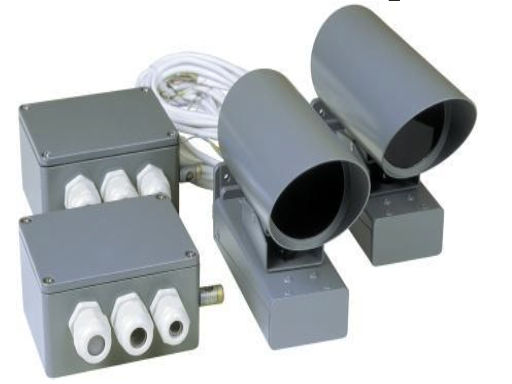
\includegraphics[height=0.20\textheight,valign=t]{my_folder/images//infr.png} %высоту рисунка выставили как 0,3 от высоты наборного поля
	\end{subfigure}
%	\hfill %выровнять по ширине
	\adjustbox{minipage=1.3em,valign=t}{\subcaption{}\label{fig:izvesh}}%
	\begin{subfigure}[t]{\dimexpr.5\linewidth-1.3em\relax}%разрешили выделить 0,5 стр в ширину на рисунок
		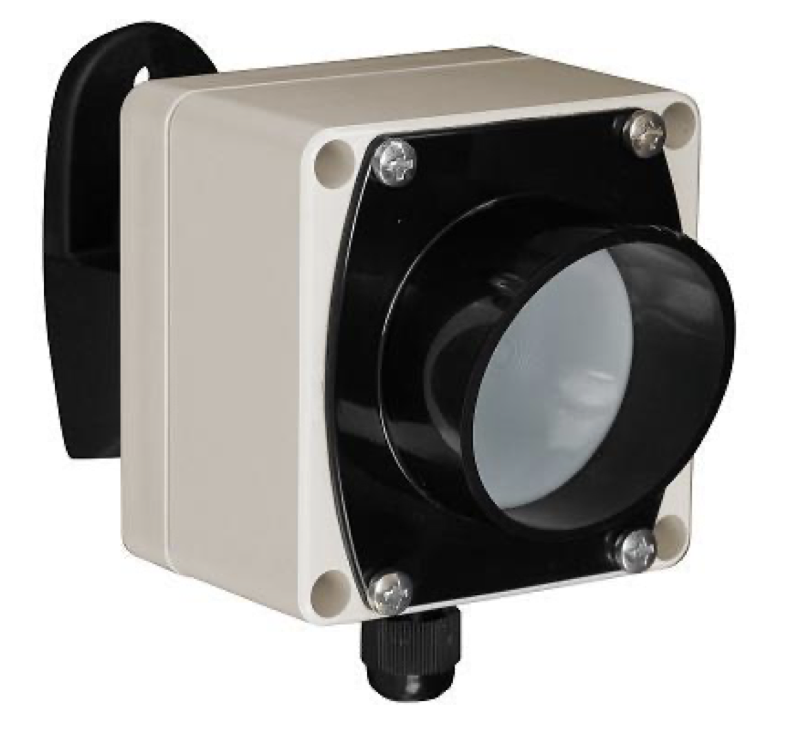
\includegraphics[height=0.20\textheight,valign=t]{my_folder/images//izvesh.png}%высоту рисунка выставили как 0,3 от высоты наборного поля
	\end{subfigure}
\captionsetup{justification=centering} %центрировать
	\caption{Примеры систем охраны периметра: {\itshape a} --- активный инфракрасный извещатель; {\itshape b}~--- уличный цифровой оптико-электронный пассивный инфракрасный излучатель}\label{fig:two_izvesh} 
\end{figure}

Каждое из этих технических средств обладает своими преимуществами и особенностями, которые определяют их использование в зависимости от конкретных требований объекта охраны. Комплексное применение различных типов извещателей позволяет создавать многоуровневую систему безопасности, способную эффективно противостоять различным видам угроз.

%\section{Задача локализации грузовых автомобилей в целях обеспечения безопасности}

\section{Выводы} \label{ch1:conclusion}
Представленные методы обеспечения охраны территорий, включая инженерно-технические средства, системы видеонаблюдения, контроля доступа и сигнализации, представляют собой многообразные и технологически продвинутые решения для предотвращения несанкционированного доступа и защиты объектов. Однако, несмотря на их эффективность и многоуровневый подход, эти методы имеют ряд существенных недостатков и ограничений.

Физическая охрана и технические средства требуют значительных финансовых затрат на установку, обслуживание и модернизацию. Они также зависят от человеческого фактора, что может привести к ошибкам и нарушениям безопасности. Инженерно-технические заграждения, которые обеспечивают физические барьеры, не всегда могут реагировать на динамические угрозы и требуют постоянного мониторинга.

Системы контроля доступа и сигнализации обеспечивают высокий уровень защиты, но часто сложны в интеграции и эксплуатации. Они требуют постоянного обновления и адаптации к новым угрозам и технологиям. Более того, в случае кибератак или технических сбоев эти системы могут быть выведены из строя, что существенно снижает уровень безопасности.

Таким образом, представленные методы, хотя и обеспечивают базовый уровень защиты, не всегда могут эффективно и оперативно реагировать на угрозы. Для повышения уровня безопасности необходимо разрабатывать и внедрять автономные интеллектуальные методы охраны территорий. Такие системы, основанные на искусственном интеллекте и машинном обучении, способны самостоятельно анализировать большие объемы данных, предотвращать потенциальные угрозы, адаптироваться к изменяющимся условиям и минимизировать зависимость от человеческого фактора. Интеллектуальные системы охраны могут значительно повысить уровень безопасности, обеспечивая более надежную и устойчивую защиту объектов в современных условиях.